\documentclass[thesis.tex]{subfiles}
\begin{document}

\chapter{Related Work}
\label{chap:prevwork}

% Categories from GISTAR
% * Finite Elements (also contains voxel based GI)
% * Monte-Carlo ray tracing
% * Photon Mapping
% * Instant Radiosity
% * Many lights (hierarchical! gathering of lights)
% * Point-based (render points somehow)
% * Discrete ordinate methods (propagation volumes etc.)
% * Precomputation

This chapter gives an overview of related realtime global illumination techniques.
Ritschel et al. \cite{bib:RealtimeGIOverview} already gave a great overview over this field for all approaches before 2012.
Therefore, we will focus on newer methods and those which are either fundamental, similar or inspirational to this thesis instead of trying to cover the whole field.

\section {Many-Lights Methods}
\begin{figure}[h]
	\centering
	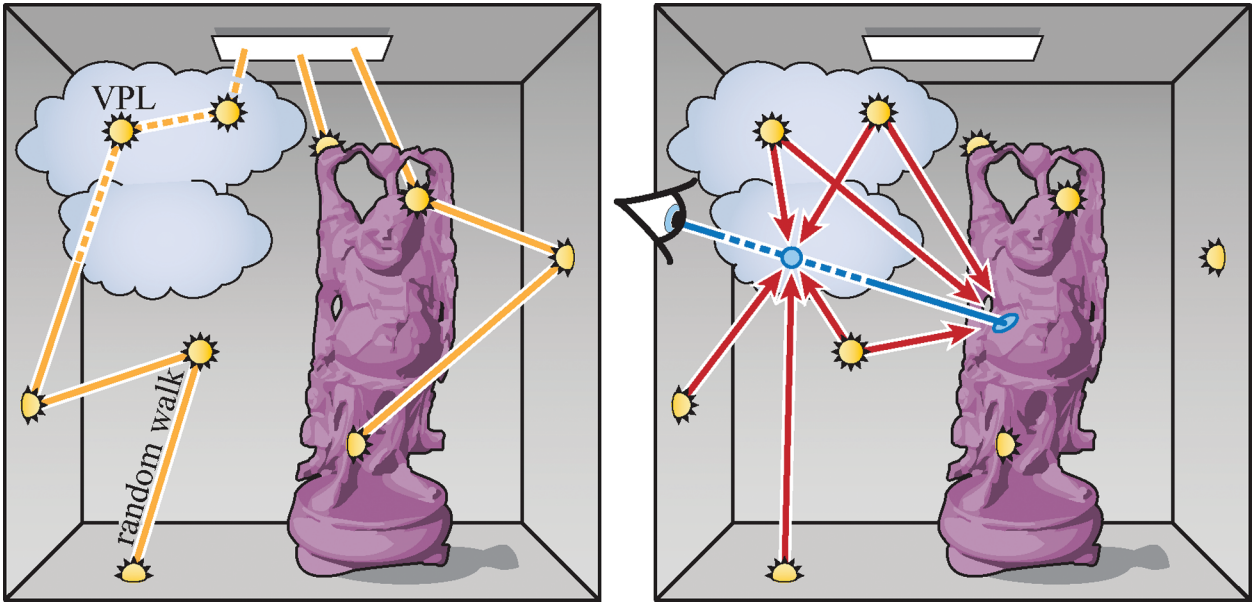
\includegraphics[width=0.8\textwidth]{manylights}
	\caption{\cite{bib:manylightssurvey2014} Two passes of many-light algorithms: Left distribution of virtual lights, right direct lighting using virtual lights.} \label{fig:manylights}
\end{figure}
Many-light methods reduce the global illumination to the smaller problem of calculating the direct lighting of many virtual light sources.
The basic principle was first described in Keller's work on Instant Radiosity \cite{bib:instantradiosity} (IR).
All many-light approaches perform two passes (see \autoref{fig:manylights}):
First virtual light sources are distributed in the scene, second each virtual light source performs direct lighting.
The main advantages of the many-light approach in general is its relatively easy unified framework and its good scalability in performance and quality.
Global illumination using $M$ virtual lights can generally be expressed as following:
\begin{equation}
L_o(\mathrm{x}, \omega_o) = \sum\limits_{i=1}^{M} f_r(\mathrm{x}, \overrightarrow{\mathrm{x}\mathrm{x}_i}, \omega_o) \cdot G(\mathrm{x}, \mathrm{x}_i) \cdot V(\mathrm{x}, \mathrm{x}_i) \cdot f_r(\mathrm{x}_i, \omega_i, \overrightarrow{\mathrm{x}_i\mathrm{x}}) \cdot \phi_i
\end{equation}
Where $G(\mathrm{x}, \mathrm{x}_i)$ is the geometry term which describes the light transfer from the virtual light in $x_i$ to the surface in point $x$.
It depends on the type of the virtual light source.
$V(\mathrm{x}, \mathrm{x}_i)$ is the visibility of a virtual light and $\phi_i$ its incoming flux.
The original IR distributes the light by tracing photon rays from the light source that are bounced inside the scene.
As also many more recent techniques, IR used virtual point light sources (VPL).

Dachsbacher et al. \cite{bib:manylightssurvey2014} did recently a detailed survey on many-lights for both offline and real-time rendering.
We focus here on the most important real-time approaches.

\subsection{Reflective Shadow Mapping}
One of the most important real-time global illumination algorithms is reflective shadow mapping by Dachsbacher et al. \cite{bib:reflectiveshadowmaps} on which many other approaches, including the one presented in this thesis, rely.
It handles the virtual light distribution with the rasterization of an extended shadow map, the reflective shadow map (RSM).
The RSM does not only contain depth as normal shadow maps, but also the reflected flux and the normal of the surface in each texel.
Each texel of this shadow map is then seen as virtual point light.
The original paper shades each pixel with a given number of sampled VPLs without taking indirect shadows into account.
Also, the technique handles only a single indirect bounce of diffuse lighting which means that a VPL is strictly speaking a hemispherical Lambert emitter.
(Like most literature we will use the term "VPL" interchangable)

While RSM offers an easy way to generate virtual lights in real-time generation of, it does basically not alter the way how those lights are applied and how their visibility is determined.
There are a few techniques that try to reduce the number of virtual lights and create few virtual area lights (VAL) by clustering
Both Dong et al. \cite{bib:clusturedvisiblity:dong} and Prutkin et al. \cite{bib:clusturedvisiblity:prutkin} suggest to cluster VPLs using k-means.
The former performs the clustering in world-space, the later directly in image space of the RSM.
Both approaches suffer from temporal coherence problems since the size and position of the clusters can change rapidly.

\subsection{VPL Bias and Compensation}
Using virtual point lights, the geometry term is defined as following:
\begin{align}
G(\mathrm{x}, \mathrm{x}_i) = \frac{(\hat{\mathbf{n}} \cdot \overrightarrow{\mathrm{x}\mathrm{x}_i} )^+}{||\mathrm{x} - \mathrm{x}_i||^2} \cdot (\hat{\mathbf{n}}_i \cdot \overrightarrow{\mathrm{x}_i\mathrm{x}})^+
\end{align}
Where $\mathbf{n}$ and $\mathbf{n}_i$ are the surface normals in point $\mathrm{x}$ and $\mathrm{x}_i$ respectively.
Note that the geometry term is a combination of the photometric distance law (fraction of cosine of angle to light source and squared distance to light source) and the definition of intensity for Lambert emitter (cosine of angle to receiver) as described earlier in \autoref{sec:preq:theo:relation}.
\\
\begin{figure}[h]
\centering
\begin{subfigure}[b]{0.48\textwidth}
	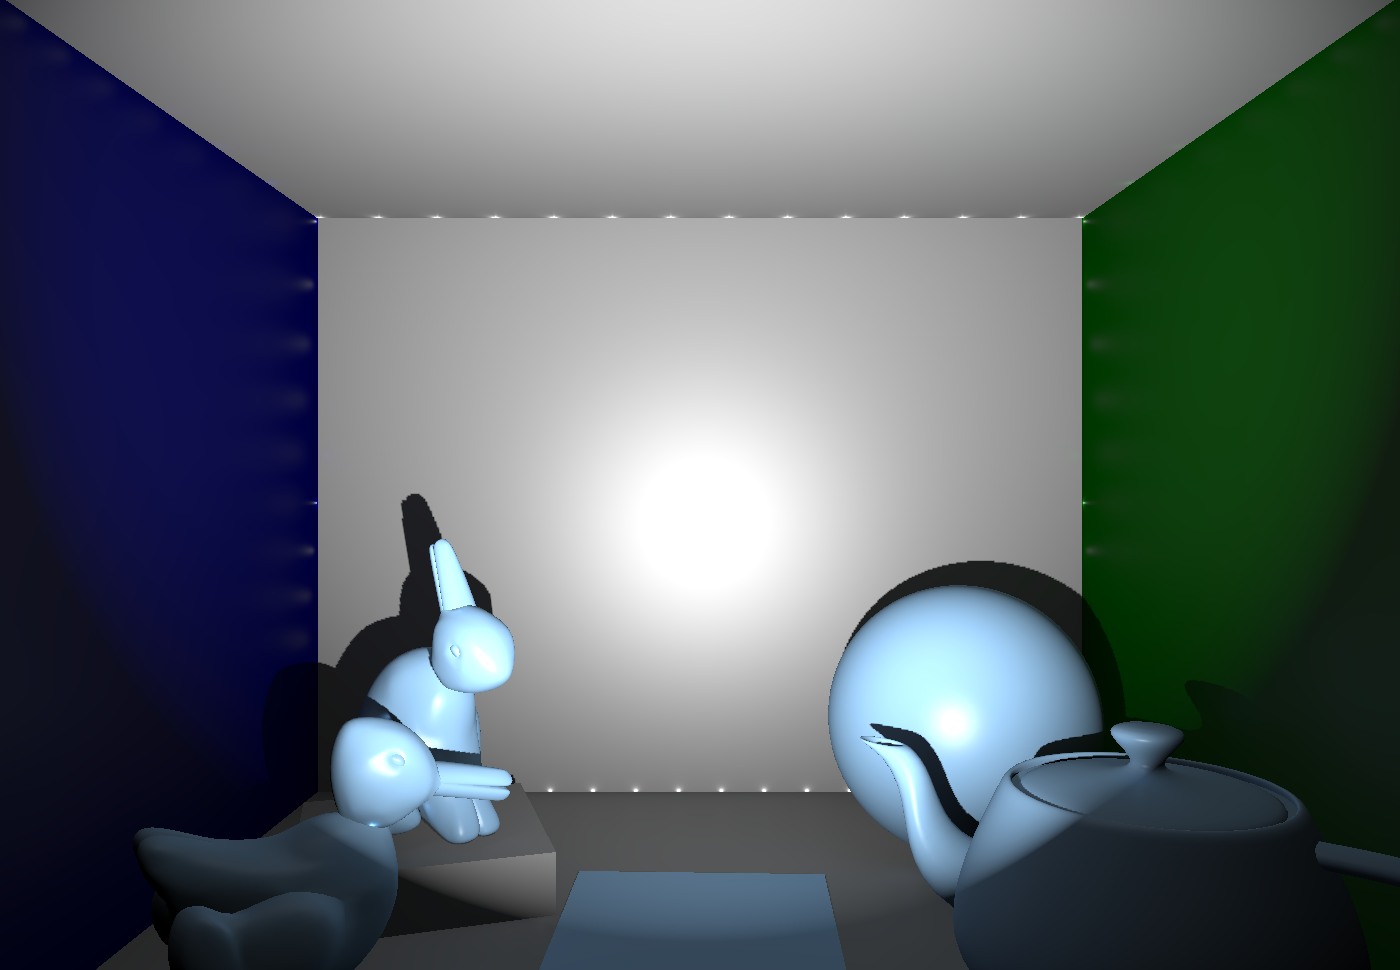
\includegraphics[width=\textwidth]{rsmbias/default}
\end{subfigure}
\begin{subfigure}[b]{0.48\textwidth}
	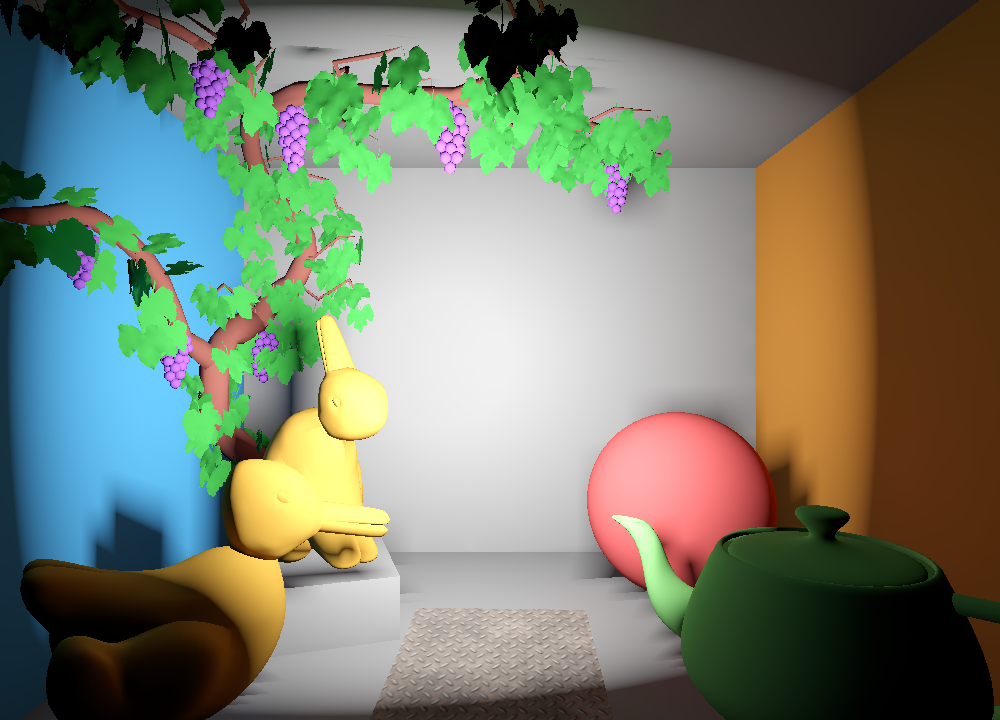
\includegraphics[width=\textwidth]{rsmbias/val}
\end{subfigure}
\caption{Left: Small bright splotches due to inverse squared distance in geometry term. Right: Using virtual area lights as proposed in \cite{bib:LightskinPaper}.}\label{fig:rsmbias}
\end{figure}
The inverse-squared distance between shading point and light source introduces a singularity, as this distance is zero in the limit.
Therefore, the contribution of a VPL reaches infinity in such a point.
The result are bright splotches, mostly visibility in creases, as seen left in \autoref{fig:rsmbias}.

Typically these artifacts are avoided by clamping the geometry term to a user defined maximum which obviously introduces a bias.
There are several bias compensation techniques:
Kollig and Keller \cite{bib:biascomp:kk04} shoot rays to nearby surface and evaluate the lighting there to transport it back to the original surface.
However, this technique may degenerate to path-tracing is thus not suitable for interactive applications.
Other techniques try to compensate the bias approximately.
For example the bias compensation by Nov\'{a}k et al. \cite{bib:biascomp:novak11} stores the bounded transport in screen-space and computes then residual transport.
Although it misses invisible surfaces, it is both efficient and plausible in its results.
\\
There are also several approaches that use different types of virtual light sources instead of VPLs.
Ha{\v{s}}an et al. \cite{bib:biascomp:vsl} introduce a new light type, the virtual spherical light (VSL).
Instead of a point-to-point evaluation, this allows them to integrate over the solid angle subtended by the spherical light sources.
Their approach is biased but does not cause bright splotches and preserves the overall energy by redistributing.
\\
Lensing et al. \cite{bib:LightskinPaper} use approximate disc shaped lights.
Since they use reflective shadow maps, the area of these virtual areal lights $A_{VAL}$ can easily be estimated by the distance of the VAL to the light source and the solid angle a RSM texel subtends.
They show that if all surfaces are assumed to be diffuse, the lighting can be solved analytically by a simple change in the geometry term:
\begin{align}
G(\mathrm{x}, \mathrm{x}_i)_{VAL} = \frac{(\hat{\mathbf{n}} \cdot \overrightarrow{\mathrm{x}\mathrm{x}_i} )^+}{||\mathrm{x} - \mathrm{x}_i||^2 + A_{VAL}} \cdot (\hat{\mathbf{n}}_i \cdot \overrightarrow{\mathrm{x}_i\mathrm{x}})^+
\end{align}
Using this geometry term, splotches at specular surfaces with low roughness can still occur.
However, most singularities are no longer visible (see \autoref{fig:rsmbias} right).
We use this technique in our approach since it is extremely fast, easy to implement and more plausible than a bounded geometry term.

Bias compensation in participating media are considerably more complex but not handled in this thesis.

\subsection{Shadows for Many-Lights}
Computing visibility for a large number of virtual lights is a difficult problem for realtime renderer since classic shadow computations like shadow mapping are far to expensive for this task.
There are a few methods that try to optimize shadow mapping for rendering large amount of lights:
\\
Imperfect shadow maps Ritschel et. al. \cite{bib:imperfectshadowmaps} leverages the fact that exact secondary visibility is not needed.
First points are placed at random locations on the scene geometry.
Shadow maps are then computed using these points instead of triangles which is much faster.
Holes in the shadow maps are filled with a push-pull heuristic.
The succeeding paper \cite{bib:imperfectshadowmaps:adapative} makes the technique (both VPL placement and shadowing) view adaptive and allows larger scenes.
\\
Olsson et al. \cite{bib:virtualshadowmaps} stores shadow maps on a large virtual texture and decides for each frame which lights actually need to compute shadow maps, how high their resolution should be and which objects act as occluders.
All these operations are performed on the GPU.

Other methods like Micro-rendering by Ritschel et al. \cite{bib:microrendering} or ManyLoDs by Holländer et al. \cite{bib:manylods} use hierarchical data structures to be able to render objects at the exactly needed detail.
This allows very fast approximations of visibility.
However, these techniques have also several other implications for example on how shading performed which is why they are often separately categorized as \emph{point-based GI}.

%\subsection{Shading}
%Multi-resolution splatting techniques ([All Nichols] Hierarchical
%image-space radiosity for interactive global illumination, Multiresolution splatting for indirect illumination, Interactive indirect illumination using adaptive multiresolution splatting) are not as efficient as "Tiled Deferred Shading" (according to \cite{bib:clusturedpreconvoledradiancecaching} (where it is just a side note!)) ... logically Tiled Deferred Shading is even better.
%Interleaved Sampling (Interleaved sampling. In
%Proc. of Eurographics Workshop on Rendering (2001)) also a good idea 
%
%Clustured Forward/Deferred Shading: Finding Unique clusturs is DIFFERENT in paper \cite{bib:clusturedshading} and practical implementation like "Pratical Clustured Shading" (SIGG2013, Humus). Paper uses (local) sorting and page tables. Humus uses Volume Texture. Ollson Siggra2013 presentation uses parallel prefix sum.
%

\section{Caching Methods}
Many recent real-time global illumination methods, including our own, compute indirect lighting only for special \emph{light caches} and interpolate the results of those across many pixels.
Which quantities a light cache saves varies from technique to technique as well as the strategies that is responsible for creating light caches either at runtime or as a pre-computation step.
Since our approach relies on dynamic cache placement, its implications and trade-offs will be discussed in \autoref{sec:impl:dyncacheplace}.

\subsection{(Irr-)Radiance Caching}
The basic idea of light caches was first introduced by Ward et al. \cite{bib:irradiancecaching} in the form of Irradiance Caching (IC) to speed up path-tracing.
Each time a ray intersects a diffuse surface it first checks if there are nearby caches from which the irradiance can be interpolated, if not, the irradiance is computed and a new cache is created at this place.
There are many extensions to this method, most notably Radiance Caching by Krivanek et al. \cite{bib:radiancecaching} (RC) which supports arbitrary glossy surfaces by saving incoming radiance encoded in a high order spherical harmonics representation.

\begin{figure}[h]
	\centering
	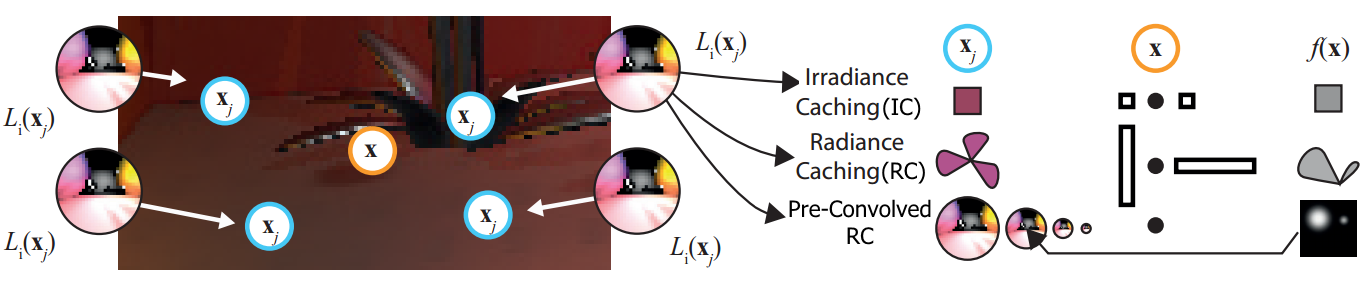
\includegraphics[width=\textwidth]{preconvolvedradiancecaching}
	\caption{\cite{bib:preconvoledradiancecaching} Storage and evaluation of pre-convolved RC in comparison with "classic" IC/RC.
	IC store a single value,
	RC store a series of SH components,
	pre-convolved RC store mipmaps of incoming radiance.} \label{fig:preconvolvedradiancecaching}
\end{figure}
Pre-convoled Radiance Caching by Scherzer et al. \cite{bib:preconvoledradiancecaching} is able to perform radiance caching with a single indirect bounce at interactive frame-rates.
As in the original radiance caching, caches lie on surface.
Each cache renders a hemisphere of all incoming radiance values as depicted in \autoref{fig:preconvolvedradiancecaching}.
The result is then pre-convolved using mipmapping to be able to evaluate quickly arbitrary specular exponents (the paper makes use of the Phong BRDF).
Caches are placed statically and apply their results using splatting, i.e. rendering them directly to a deferred shading buffer.
Clustured Pre-Convolved Radiance Caching, an extension to the previous method by Rehfeld et al. \cite{bib:clusteredpreconvoledradiancecaching}, places the radiance caches according to screen-space clusters which makes the technique more scalable but less temporal coherent.
Additionally it uses cone tracing (which will be explained in \autoref{sec:prev:voxelmethods}) in a prefiltered voxel instead of rasterization to render the cache's radiance hemispheres.

\subsection{(Irr-)Radiance Volumes}
\begin{figure}[h]
	\centering
	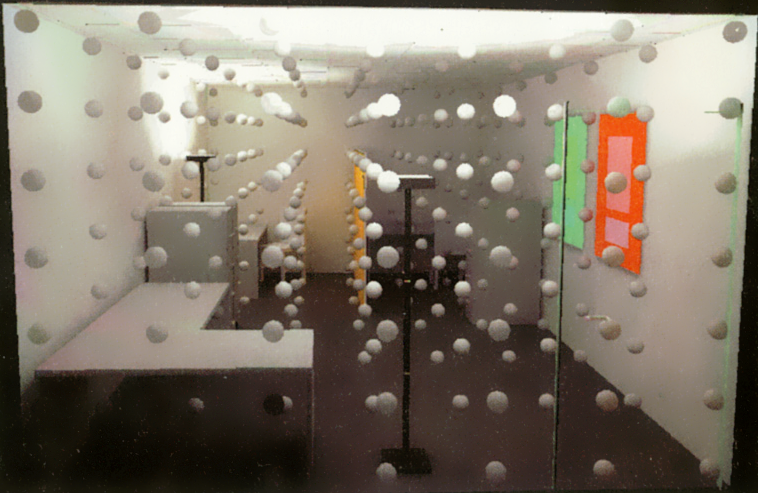
\includegraphics[width=0.7\textwidth]{gregerirradiancevolume}
	\caption{\cite{bib:irradiancevolume} Visualization of an irradiance volume. Each sphere visualizes a light cache colored by the local irradiance for each direction. } \label{fig:irradiancevolume}
\end{figure}
Irradiance volumes as proposed by Greger et al. \cite{bib:irradiancevolume} are very popular to light dynamic objects in otherwise static environments.
An irradiance volume is a regular grid in which each grid cell saves precomputed irradiance values for all directions.
The original work uses hemispherical grid mappings to save irradiance values.
However, other representation like spherical harmonics are common in praxis.
Objects to be lit can then use their normal vectors to look-up the precomputed irradiance values to perform diffuse lighting.
Note however that this method can does not handle light bounced off or occluded by dynamic objects.

The advantage of saving irradiance for all possible normals over saving incoming radiance for each direction, is that an irradiance signal has a much lower frequency than radiance.
Only a single irradiance value is needed for diffuse lighting of a surface (i.e. a given normal) which is equivalent to a hemispherical integration over the incoming radiance.
Nonetheless, if arbitrary BRDFs are to be supported, the total incoming irradiance for a given normal is not sufficient and integration over radiance is necessary.
Note however, that for a spherical harmonics representations, integration over a lobe given in SH has the same costs as evaluating the SH coefficients for a certain direction (as earlier described in \autoref{sec:preq:shprojectrecon}).

Njasure et al. \cite{bib:nijasure:rtirradiancevol} compute radiance volumes at runtime with interactive frame rates by rendering a cubemap at each grid point and compute a low number of spherical harmonics coefficients from each of them.

\subsection{Other Real-Time Caching-Based Methods}\todo{awful section name}

Radiance Hints \cite{bib:radiancehints}.

Real/time radiance caching http://jcgt.org/published/0003/04/06/ \cite{bib:radiancecachechromaticcompression}
Meep! This paper sees itself as extension to Radiance Hints!

LightSkin \cite{bib:LightskinPaper} of Lensing et. al.


\section{Discrete Ordinate Methods}
Discrete ordinate methods compute light transport by exchanging energy between a cellular discretization of the scene.
Usually it is possible to update the lighting iteratively across many frames.
As long as there are no high frequency changes, slow adaption can exploit frame coherencies to benefit the overall performance drastically.

% % % % % % % % % % % % % % % % % % % % % % % % % % % % % % % % % % % % % % % % % % % % % % % %
\begin{figure}[h]
\centering
\begin{subfigure}[b]{0.35\textwidth}
\centering
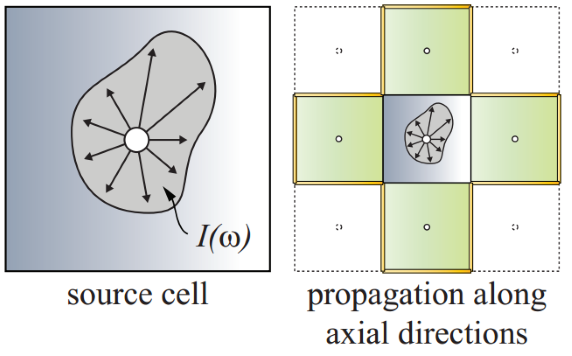
\includegraphics[width=\textwidth]{lpv/principle}
\caption{Light propagation principle.}
\label{fig:lpv:principle}
\end{subfigure}
\begin{subfigure}[b]{0.53\textwidth}
\centering
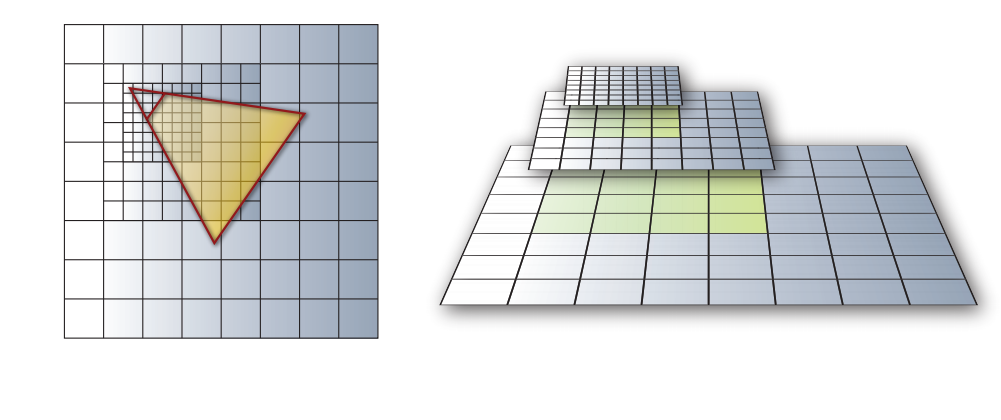
\includegraphics[width=\textwidth]{lpv/cascading}
\caption{Cascading of multiple LPVs.}
\label{fig:lpv:cascading}
\end{subfigure}
\\
\begin{subfigure}[b]{\textwidth}
\centering
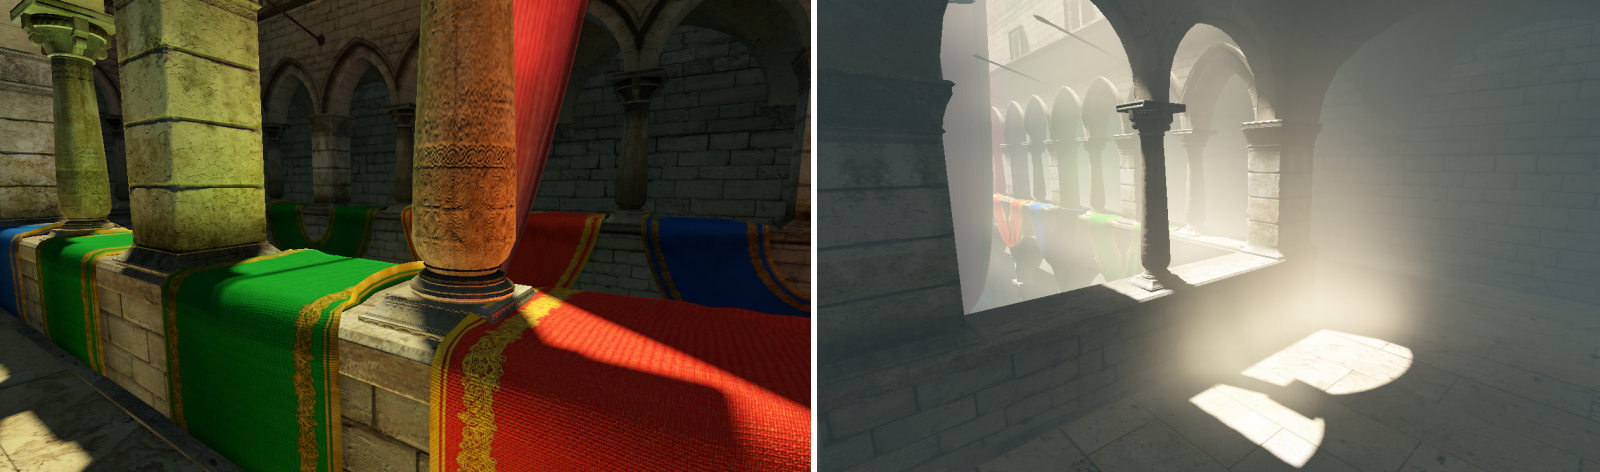
\includegraphics[width=\textwidth]{lpv/results}
\caption{Left: Low frequency indirect lighting. Right: Lit participating media.}
\label{fig:lpv:results}
\end{subfigure}
\caption{\cite{bib:lpt} Cascaded LPV, principles and results.}
\end{figure}
% % % % % % % % % % % % % % % % % % % % % % % % % % % % % % % % % % % % % % % % % % % % % % % %
A popular real-time representative of these methods is Cascaded Light Propagation Volumes by Kaplanyan and Dachsbacher \cite{bib:lpt}.
Using a RSM, light is injected into a light propagation volume (LPV).
The LPV is a regular grid where each cell contains a light intensity distribution represented by a few low order spherical harmonic coefficients.
A second grid stores a volumetric representation used for fuzzy occlusion.
Considering these blockers, the light is then propagated across the LPV in each frame (see \autoref{fig:lpv:principle}).
For better scalability with larger scenes, multiple nested LPVs are used as visualized in \autoref{fig:lpv:cascading}.
After the propagation, the LPVs can easily be used to light the scene.
The approach does not rely on any pre-computation and is able to capture both diffuse and low frequency specular lighting in real-time (see \autoref{fig:lpv:results}).
However, it is very prone to light bleeding artifacts (light "seeping" incorrectly through blockers) and depending on the LPV resolution light may only be transported for rather short distances.
\\
The original approach obtained the blocker volume from the already existing information in RMS and the camera view.
Rasterized Voxel-based GI by Doghramachi \cite{bib:rasterizedvbgi} presents an alternative real-time voxelization approach alongside with several implementation improvements.

\todo{more discrete ordinate methods or rename section}

\section{Voxel-Volume-Tracing Methods} \label{sec:prev:voxelmethods}

Voxel GI

\todo{original voxel cone tracing} Has been evaluated in game engines. "MITTRING M.: The Technology Behind the Unreal Engine 4 Elemental demo. SIGGRAPH 2012 Advances in RealTime Rendering in 3D Graphics and Games Course, 2012." 

Layered Reflective Shadow Maps for Voxel-based Indirect Illumination decouples occlusion from lighting data.
Visibility determination is handled via Voxel Cone tracing while the actual lighting is performed by lookups in a pre-filtered Layered Reflective Shadow Map.
Doing so avoids most of the memory and initialization/update overhead associated with the large voxel data structure, since each voxel encodes only binary visibility information.
Layers to avoid discontinuities, etc.

\subsection{Voxelization}

\cite{bib:GPUGems2}[Chapter 42] $http://http.developer.nvidia.com/GPUGems2/gpugems2_chapter42.html$

Modern GPU in OpenGL Insights \cite{bib:openglinsightsvoxel}

Maxwell GPUs per Hardware

\section{Summary}
Metabla\\
RSM important\\
Which methods fulfill goals of this thesis

\subfilebib % Makes bibliography available when compiling as subfile
\end{document}